
% This LaTeX was auto-generated from MATLAB code.
% To make changes, update the MATLAB code and republish this document.

\documentclass{article}
\usepackage{graphicx}
\usepackage{color}

\sloppy
\definecolor{lightgray}{gray}{0.5}
\setlength{\parindent}{0pt}

\begin{document}

    
    \begin{verbatim}
clear;close all;clc;


freq=8000;
Ts=1/freq;
ws=2*pi*freq;fc=2000;bw=2*pi*fc;w0=bw;
w1=0:1:2*bw ;
n=1:length(w1);
x(n)=1;
l=1;
fOrder = 1;



i = true;
while(i)
    S=0;
for  w=0:1:bw

      s=1i*w/w0;

    H = butterWorth(fOrder,w,w0);


     S=S+(abs(H))^2;

end



arr=[-6 -5 -4 -3 -2 -1 1 2 3 4 5 6 ];

%  arr = -6:6;
Noise=0;


for  w=0:1:bw
N =0;




     for  n=1:10

          k=w+arr(n)*ws;

         s=1i*k/w0;
         H = butterWorth(fOrder,k,w0);

          N=N+H;

     end


      Noise=Noise+(abs(N))^2;

 end



 SNR=10*log10(S/Noise);
 if SNR >= 60
     i = false;
 else
     fOrder = fOrder+1;
 end
end

fque = -10000:100:10000;
w = 2*pi*fque;
s=1i*w/w0;
B = zeros(1,length(w));
for i= 1:length(w)
    H = butterWorth(fOrder,w(i),w0);
    B(i) = H;
end



figure(1)
subplot(2,1,1)
plot(fque,abs(B));
grid on
subplot(2,1,2)
plot(fque,angle(B),'r');
grid on

fque = -10000:100:10000;
V = zeros(1,length(w));
for i= 1:length(w)

    H =  butterWorth(fOrder,(w(i)-3*ws),w0)+ butterWorth(fOrder,(w(i)-2*ws),w0)+ butterWorth(fOrder,(w(i)-1*ws),w0)+ butterWorth(fOrder,w(i),w0)+ butterWorth(fOrder,(w(i)+1*ws),w0)+butterWorth(fOrder,(w(i)+2*ws),w0)+butterWorth(fOrder,(w(i)+3*ws),w0);
    V(i) = H;
end

figure(2)
subplot(2,1,1)

plot(fque,abs(V))
ylim([0,1.5])
grid on
subplot(2,1,2)
plot(fque, angle(V))
grid on

%%%%%%%%%%%%%%%%%%%%%%%%%%%%%%%%%%%%%%%

H_dsp = sawtooth(w/8000,0.5);
H_dsp = (1-H_dsp)/2;
figure(3)
plot(fque,H_dsp)

X4 = (H_dsp).*(V);
subplot(2,1,1)
plot(fque,abs(X4));
grid on;
subplot(2,1,2)
plot(fque,angle(X4));
grid on;

S_H =sinc(fque/8000);

X5 = X4.*S_H;
figure(7)
subplot(2,1,1)
plot(fque,abs(X5));
grid on;
subplot(2,1,2)
plot(fque,angle(X5));
grid on;
%%%%%%%%%%%%%%%%%%%%%%%%%%%%%%%
SNR_Jitter = 60;
T_signal = 1/2000;
T_jitter = (0.194*T_signal)/sqrt(SNR_Jitter)
%%%%%%%%%%%%%%%%%%%%%%%%%%%%%%%%%%%%%%%%%%%%
n_bits = 12;
SNR_quant = 20*n_bits*log10(2)
i =0
freqq = -200:200;
freqq = freqq.*100;
H_r = zeros(1,length(freqq));
for i = (find(freqq == -2000):find(freqq == 2000))
    H_r(i) = 1./sinc(freqq(i)/8000);
end
figure(8)
plot(freqq,abs(H_r));
grid on;
X5 = [ones(1,100) X5 ones(1,100)];
X6 = X5.*H_r;
figure(9)
subplot(2,1,1)
plot(freqq,abs(X6));
grid on;
subplot(2,1,2)
plot(freqq,angle(X6));
grid on;
\end{verbatim}

        \color{lightgray} \begin{verbatim}
T_jitter =

   1.2523e-05


SNR_quant =

   72.2472


i =

     0

\end{verbatim} \color{black}
    
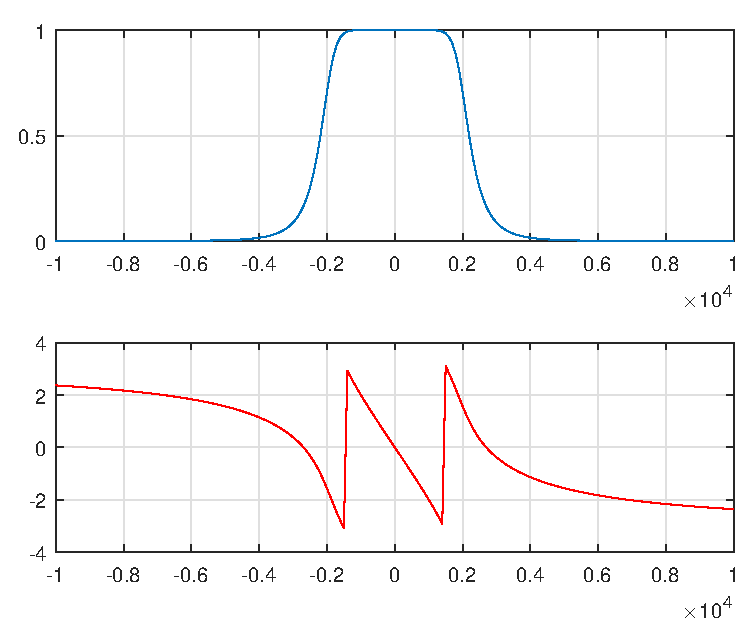
\includegraphics [width=4in]{Project1_01.eps}

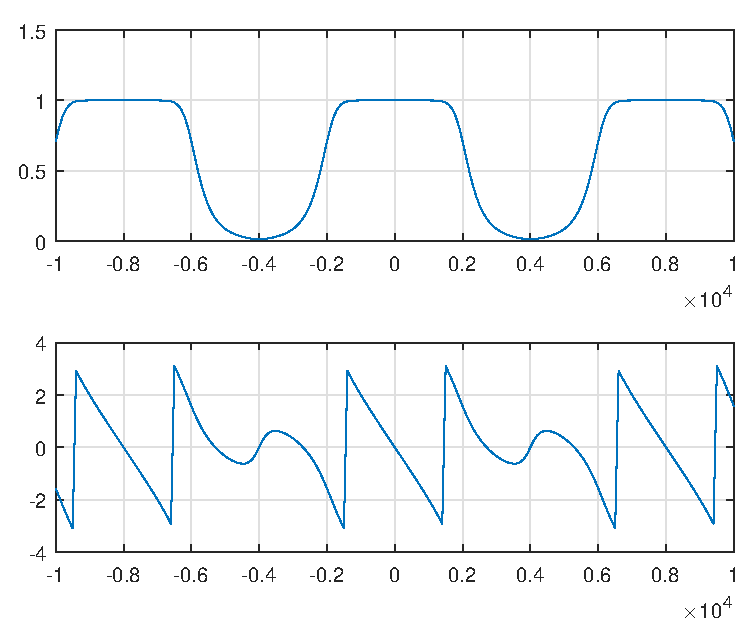
\includegraphics [width=4in]{Project1_02.eps}

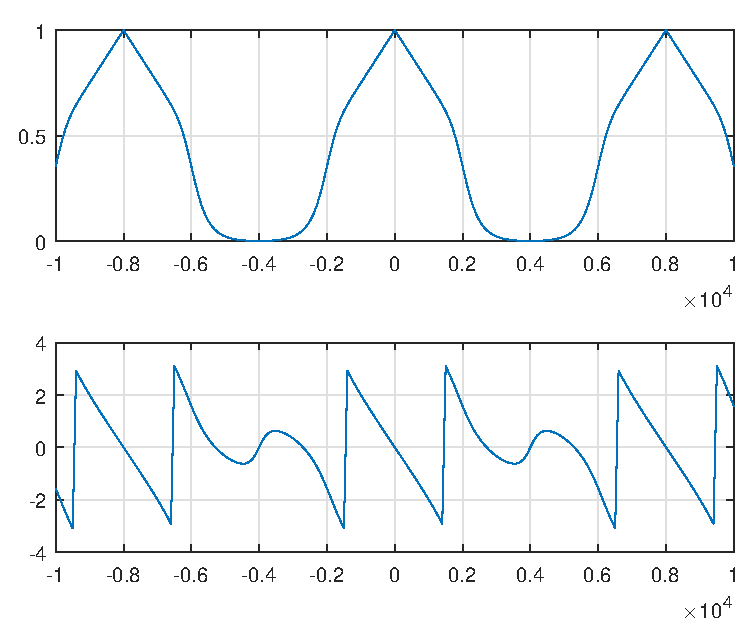
\includegraphics [width=4in]{Project1_03.eps}

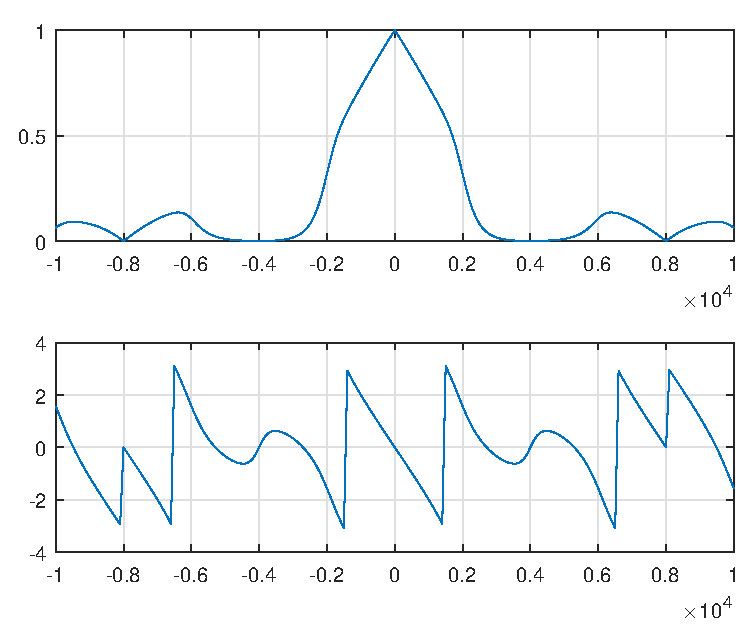
\includegraphics [width=4in]{Project1_04.eps}

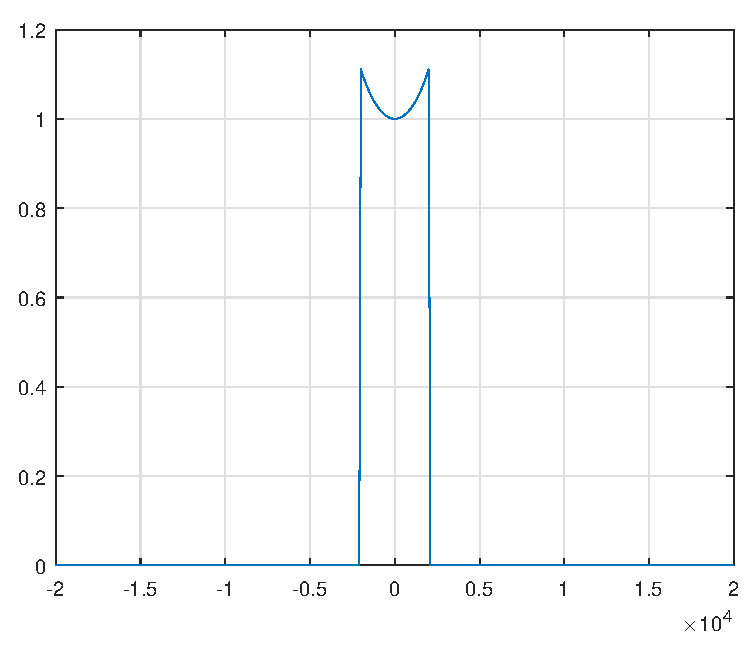
\includegraphics [width=4in]{Project1_05.eps}

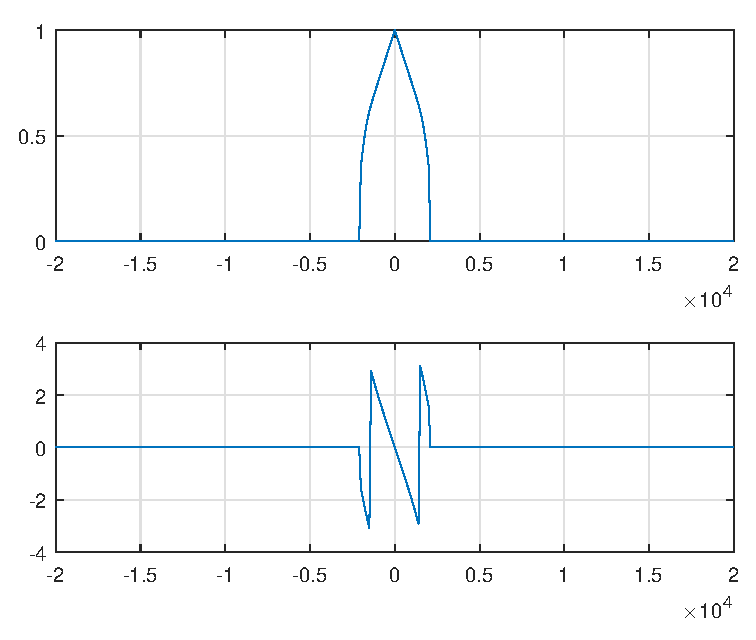
\includegraphics [width=4in]{Project1_06.eps}



\end{document}
    
